%\newpage
\appendix
%\appendixpage\dfrac{num}{den}

% appendix start here  % appendix start here  % appendix start here  
\chapter{Additional Resources}
\label{app:chapter_additional_resources}
% appendix start here  % appendix start here  % appendix start here  

\section{Doubly Robust Estimator}
\label{app:drdeep}

In this section, for completeness, I present the $\widehat{A T T}_{d r}(g, t)$ as 
described in \textcite[Section 4]{cs2021did_mtp}. Only the equations for the never-treated 
design is presented here, as this was the one used in the main analysis. Further, since
in the main analysis I do not adjust for anticipation, the version presented here
is also simplified in this respect.

\begin{equation}
    \widehat{A T T}_{d r}(g, t)=\mathbb{E}_n\left[\left(\widehat{w}_g^{\text{treat}}-\widehat{w}_g^{\text{comp}}\right)\left(Y_t-Y_{g-1}-\widehat{m}_{g, t}\left(X; \widehat{\beta}_{g, t}\right)\right)\right],
    \label{eq:attdr}
\end{equation}
where 
\begin{equation}
    \begin{aligned}[t]
        \widehat{w}_g^{\text {treat }}=\frac{G_g}{\mathbb{E}_n\left[G_g\right]},
    \end{aligned}\qquad
    \begin{aligned}[t]
        \widehat{w}_g^{\text{comp}}=\frac{\frac{\widehat{p}_g\left(X ; \widehat{\pi}_g\right) C}{1-\widehat{p}_g\left(X ; \widehat{\pi}_g\right)}}{\mathbb{E}_n\left[\frac{\widehat{p}_g\left(X ; \widehat{\pi}_g\right) C}{1-\widehat{p}_g\left(X ; \widehat{\pi}_g\right)}\right]}
        \label{eq:wgtreatcomp}
    \end{aligned}
\end{equation}

\section{TWFE Alternative Design}
\label{app:twfe}

In the following, I present the alternative model featuring a TWFE regression design. 

\begin{equation}
    Y_{i,t}=\sum_{e \in \mathcal{E}} \theta_e^{\text{\tiny{FE}}}   \mathbb{1}(\text {health degradation})_{i,t}+ \eta  X_{i,t} + \delta_i + \gamma_t + u_{i,t},
    \label{eq:twfe}
\end{equation}
where the relatvei event times $e \in \mathcal{E} = \{-10, -8, -6, -4, 0, 2, ..., 12\}$. Note that
relative event time $e=-2$ is dropped from the estimation, in order to be able to identify the ATT
in a full set of individual and year fixed effects. The indicator function $\mathbb{1}(\text {health
    degradation})_{i,t}$ tracks the relative time since/until experiencing a significant health
degradation. The vector $X$ incorporates (time varying) covariates used in the model, and $\delta_i$
and $\gamma_t$ represent the individual and year fixed effects, respectively.


\newpage

\section{Transformation of Log-Linear Specifications}
\label{sec:transformcoefs}

As explained in \code{estout}'s manual (\cite{jann2007making}),
a function, $f(b)$, and its first derivative, $\partial f(b)$, can be used to transform the coefficients to
be presented. Concretely, the following functions were used for the log specifications:  
%
\begin{equation}
    \begin{aligned}
        f(b) = 100 \cdot (e^{b}-1), 
    \end{aligned}\qquad
    \begin{aligned}
        \partial f(b) = 100 \cdot (e^{b}).
    \end{aligned}
    \label{eq:transformcoefs}
\end{equation}

According to the package's manual, the first derivative is used to transform the standard errors as in:
\begin{equation}
        \text{se} \cdot \partial f(b)
\end{equation}

With regards to the log of \textit{net} wealth, however, the original coefficients cannot be interpreted as
percentage changes due to crossing over from negative to positive and vice-versa. To illustrate, if an
individual's net worth is valued at negative $10.000$€, and in the next period it is valued at positive
$20.000$€. What would the percentage change in their net wealth? Only if one assumes very few people cross the
€0 threshold could one interpret the coefficients approximately as a percentage change. As a matter of fact,
even the interpretation of gross wealth is not, at first, trivial due to the possibility of owning 0 wealth.
This issue is, however, circumvented with the unproblematic assumption that everyone has something valued for
at least $1$€. On these accounts, the transformation was applied to both gross and net wealth specifications,
but the reader should be aware of this caveat when interpreting the results of the neglog transformation.

\newpage

\section{Health Scales and Sub-Scales Over the Life Cycle}

\begin{figure}[h]
    \begin{subfigure}{0.45\textwidth}
        \centering
        \caption{Physical Health Domain}
        \includegraphics[width=1\linewidth]{../../output/figures/validatingmcspcs/pcs_age_subscales}
        \label{fig:pcsagesubscales}
    \end{subfigure}
    \begin{subfigure}{0.45\textwidth}
        \centering
        \caption{Mental Health Domain}
        \includegraphics[width=1\linewidth]{../../output/figures/validatingmcspcs/mcs_age_subscales}
        \label{fig:mcsagesubscales}
    \end{subfigure}
    \caption{Comparison of average health summary scores and sub-scales by age group}\label{fig:bothagesubscales}
    \fnote{Notes: This figure shows the sub-scales superimposed with the summary scores constructed following the 
        SF-12 method as well as the alternative method with an oblique rotation. Since age is a key variable that
        captures most of the variation in health outcomes, this visualization helps us better grasp 
        how the summary scores behave relative to each sub-scale. Note that \textit{Mental Health} is the
        denomination of one of the sub-scales, while MCS is the summary score in the mental domain. 
        }
        { \small \vspace*{6pt}
        Panel \subref{fig:pcsagesubscales} shows the PCS (from both methodologies) and the sub-scales from the physical health dimension. 
        It becomes apparent that in this domain, the summary scores are coherent with all sub-scales in both methodologies. 
        \\ In the Mental domain, depicted in panel \subref{fig:mcsagesubscales}, one sub-scale (Mental Health) shows a different pattern to the other three. 
        MCS\tsub{sf21} follows this single variable very closely, in detriment of the other three. 
        \\ It is worth noting that the interpretation of how the mental health unfolds over the life cycle differs considerably over the two methods. 
        MCS\tsub{sf21} would suggest a rather low starting point, then a slow increase over the time, a big increase around retirement age and, finally, a rapid decrease subsequently. 
        In the oblique case, in contrast, we see a relatively high starting point, then a slow decrease over time, then only a moderate increase around retirement and, finally, also a rapid decrease later on. 
    }
\end{figure}




% bp                  Physical pain in the last 4 weeks
% gh                  Current general health
% pf1                 State of health affects ascending stairs
% pf2                 State of health affects tiring tasks
% rp1                 Accomplished less due to physical problems
% rp2                 Limitations due to physical problems
% mh1                 Run-down, melancholy in the last 4 weeks
% mh2                 Well-balanced in the last 4 weeks
% vt                  Physical pain in the last 4 weeks
% re1                 Accomplished less due to emotional problems
% re2                 Less careful due to emotional problems
% sf                  Limited socially due to health



\begin{figure}[ht!]
  A: Physical Health
  \\  %%%%%%%%%%%%%%%%%%%%%%%%%%%%%%%%%%%%%%%%%%%%%%%%%%%%%%%%%%%%%% newline 
  \begin{subfigure}{.30\textwidth}
    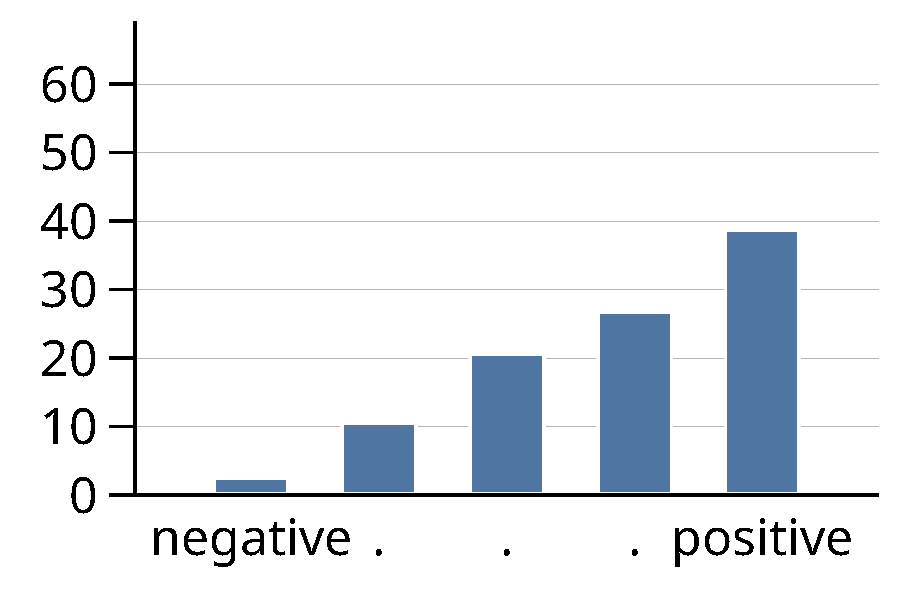
\includegraphics[width=1\linewidth]{descriptives/fig_phys_bp.pdf}
    \caption{\code{bp}: Physical pain in the last 4 weeks}
    \label{fig:bp}
\end{subfigure}\hfill%
  \begin{subfigure}{.30\textwidth}
    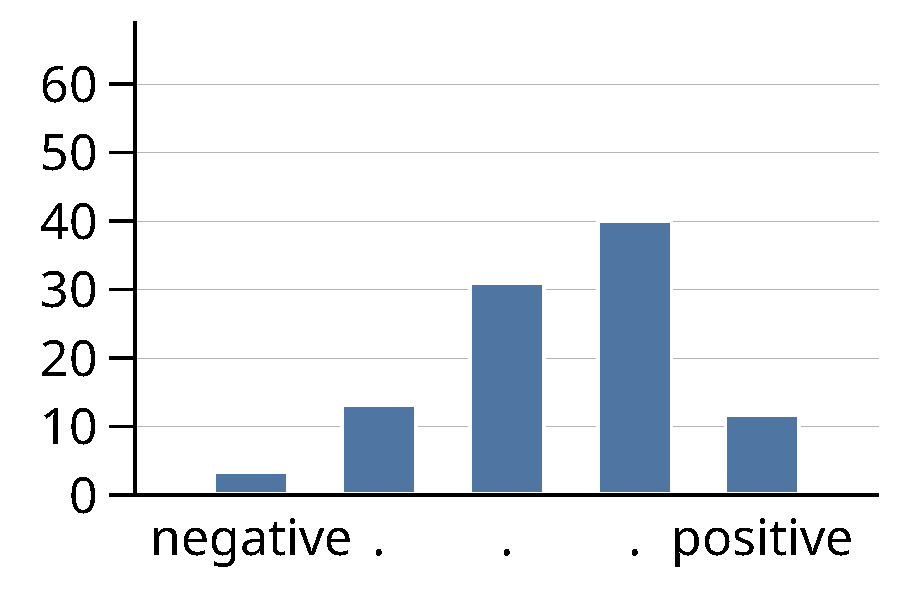
\includegraphics[width=1\linewidth]{descriptives/fig_phys_gh.pdf}
    \caption{\code{gh}: Current general health \phantom{text to break line}}
    \label{fig:gh}
\end{subfigure}\hfill%
  \begin{subfigure}{.30\textwidth}
    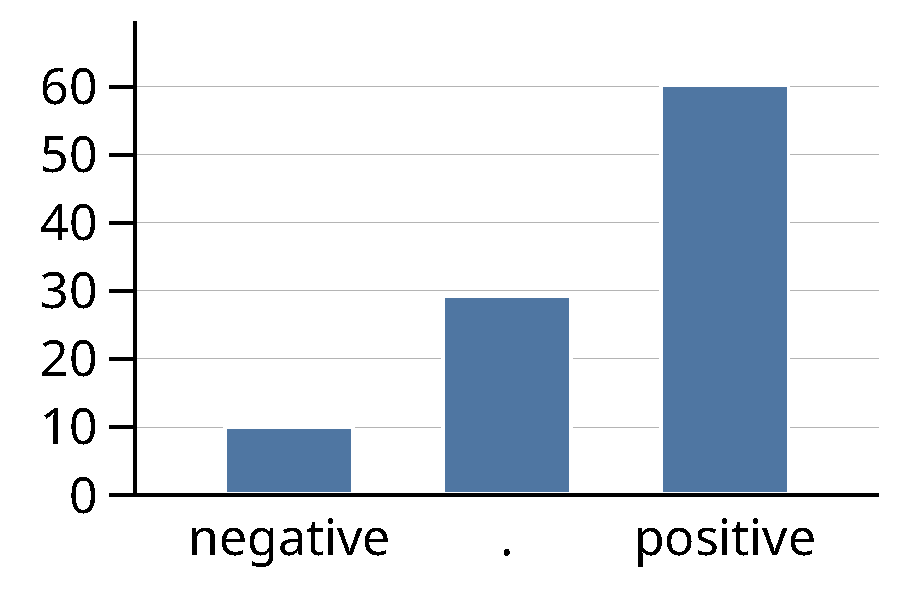
\includegraphics[width=1\linewidth]{descriptives/fig_phys_pf1.pdf}
    \caption{\code{pf1}: State of health affects ascending stairs}
    \label{fig:pf1}
\end{subfigure}\hfill%
  \\  %%%%%%%%%%%%%%%%%%%%%%%%%%%%%%%%%%%%%%%%%%%%%%%%%%%%%%%%%%%%%% newline 
  \begin{subfigure}{.30\textwidth}
    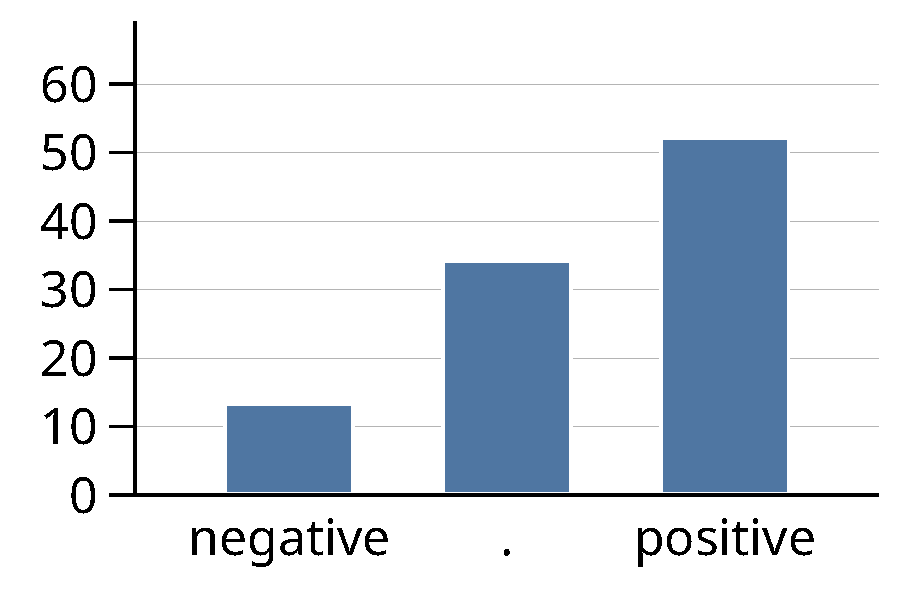
\includegraphics[width=1\linewidth]{descriptives/fig_phys_pf2.pdf}
    \caption{\code{pf2}: State of health affects tiring tasks}
    \label{fig:pf2}
  \end{subfigure}\hfill%
  \begin{subfigure}{.30\textwidth}
    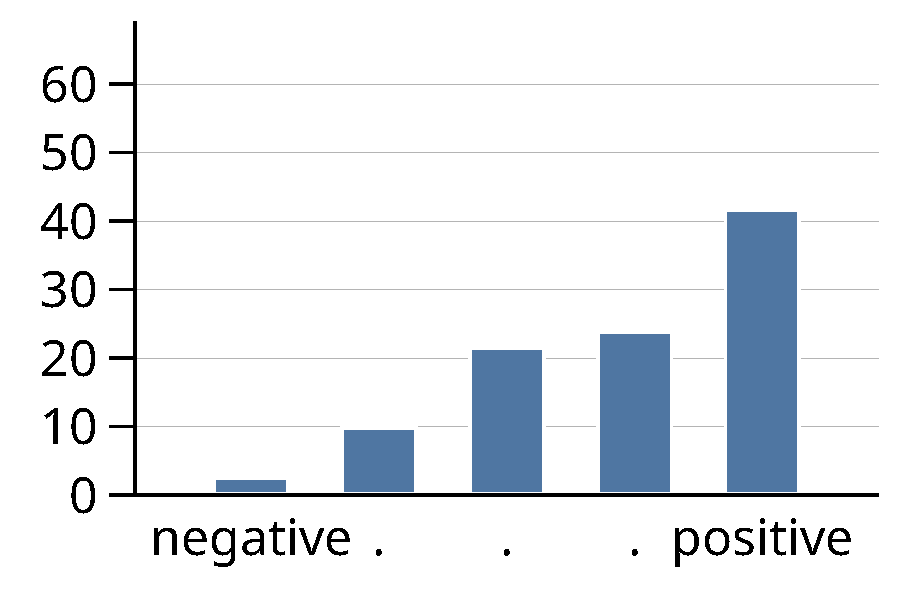
\includegraphics[width=1\linewidth]{descriptives/fig_phys_rp1.pdf}
    \caption{\code{rp1}: Accomplished less due to physical problems}
    \label{fig:rp1}
  \end{subfigure}\hfill%
  \begin{subfigure}{.30\textwidth}
    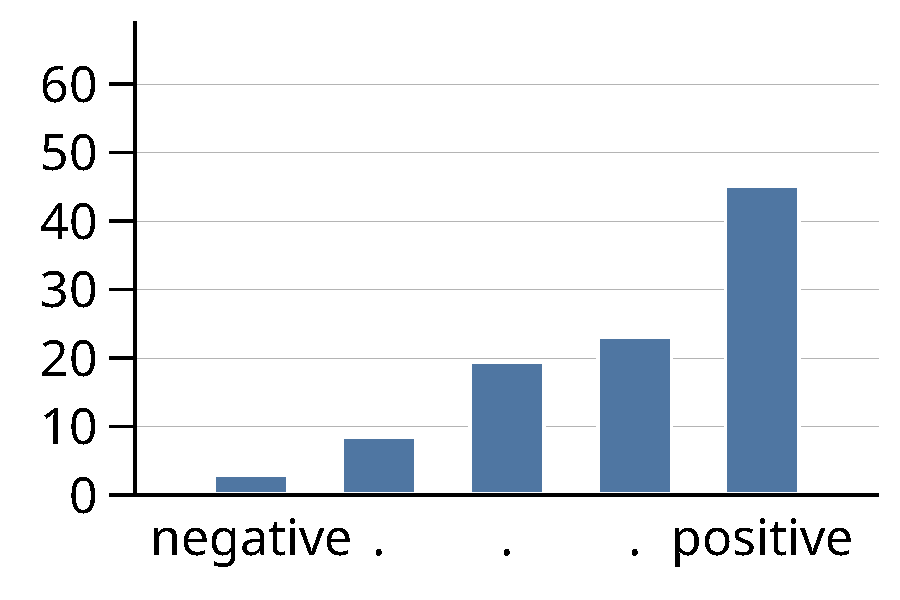
\includegraphics[width=1\linewidth]{descriptives/fig_phys_rp2.pdf}
    \caption{\code{rp2}: Limitations due to physical problems}
    \label{fig:rp2}
  \end{subfigure}\hfill%
  \\  %%%%%%%%%%%%%%%%%%%%%%%%%%%%%%%%%%%%%%%%%%%%%%%%%%%%%%%%%%%%%% newline 
  B: Mental Health
  \\  %%%%%%%%%%%%%%%%%%%%%%%%%%%%%%%%%%%%%%%%%%%%%%%%%%%%%%%%%%%%%% newline 
  \begin{subfigure}{.30\textwidth}
    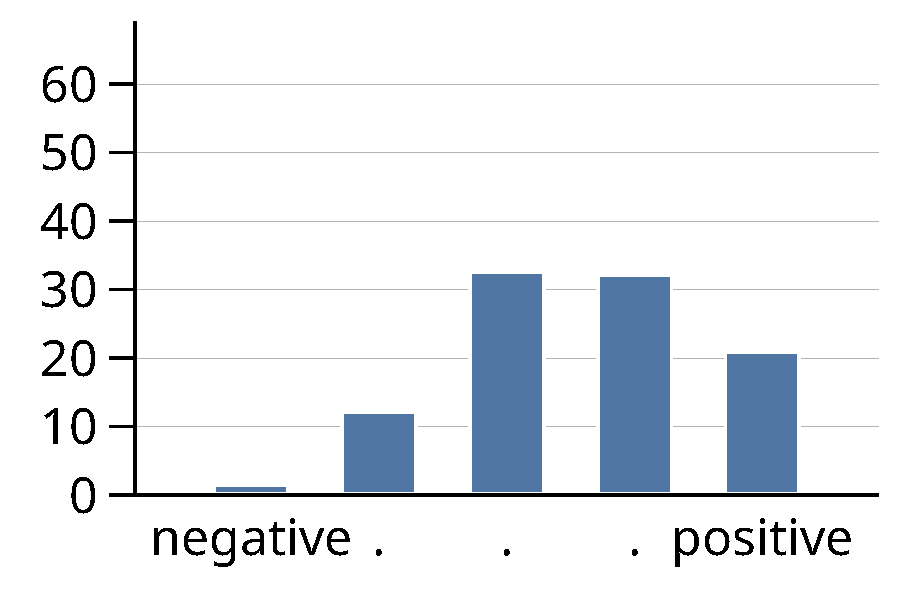
\includegraphics[width=1\linewidth]{descriptives/fig_ment_mh1.pdf}
    \caption{\code{mh1}: Run-down, melancholy in the last 4 weeks}
    \label{fig:mh1}
\end{subfigure}\hfill%
  \begin{subfigure}{.30\textwidth}
    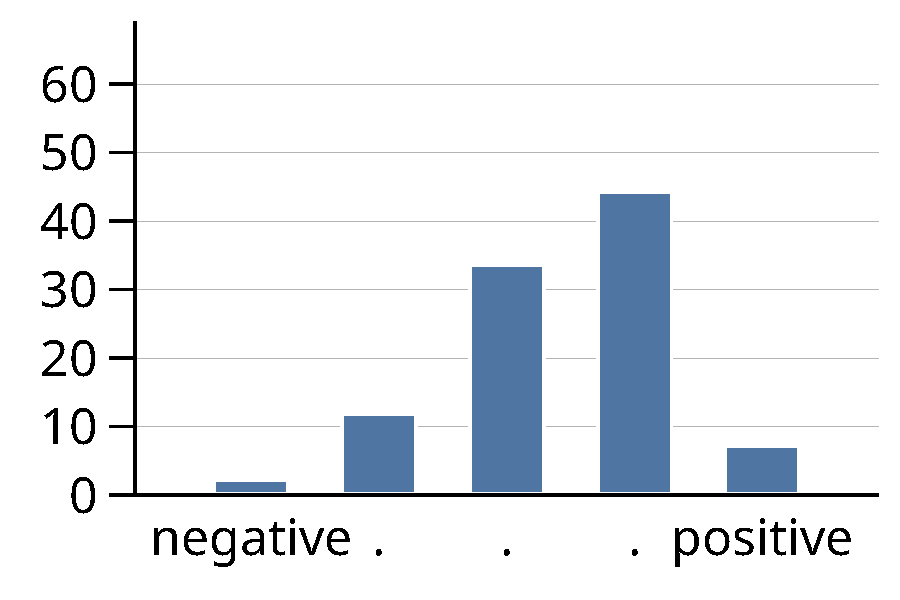
\includegraphics[width=1\linewidth]{descriptives/fig_ment_mh2.pdf}
    \caption{\code{mh2}: Well-balanced in the last 4 weeks}
    \label{fig:mh2}
\end{subfigure}\hfill%
  \begin{subfigure}{.30\textwidth}
    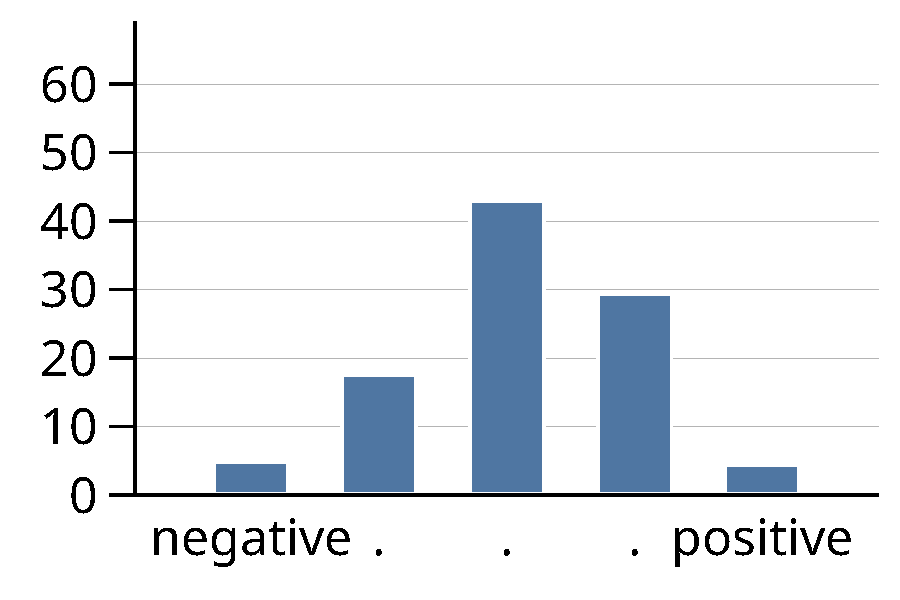
\includegraphics[width=1\linewidth]{descriptives/fig_ment_vt.pdf}
    \caption{\code{vt}: Physical pain in the last 4 weeks}
    \label{fig:vt}
\end{subfigure}\hfill%
  \\  %%%%%%%%%%%%%%%%%%%%%%%%%%%%%%%%%%%%%%%%%%%%%%%%%%%%%%%%%%%%%% newline 
  \begin{subfigure}{.30\textwidth}
    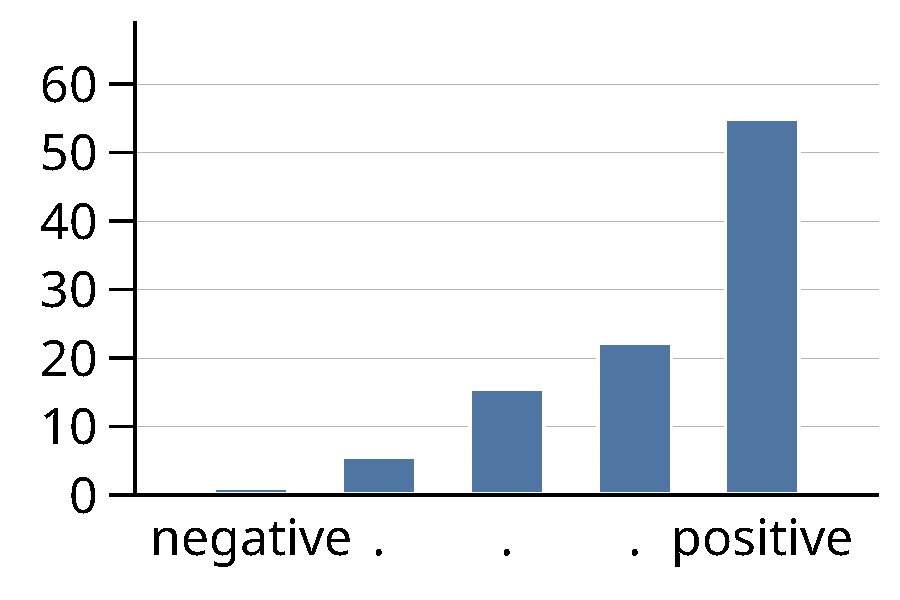
\includegraphics[width=1\linewidth]{descriptives/fig_ment_re1.pdf}
    \caption{\code{re1}: Accomplished less due to emotional problems}
    \label{fig:re1}
\end{subfigure}\hfill%
  \begin{subfigure}{.30\textwidth}
    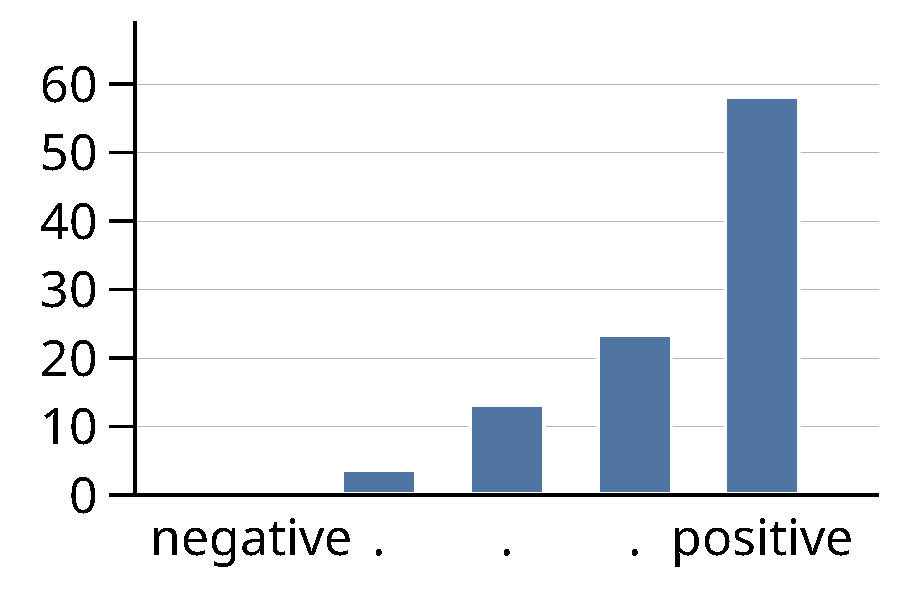
\includegraphics[width=1\linewidth]{descriptives/fig_ment_re2.pdf}
    \caption{\code{re2}: Less careful due to emotional problems}
    \label{fig:re2}
\end{subfigure}\hfill%
  \begin{subfigure}{.30\textwidth}
    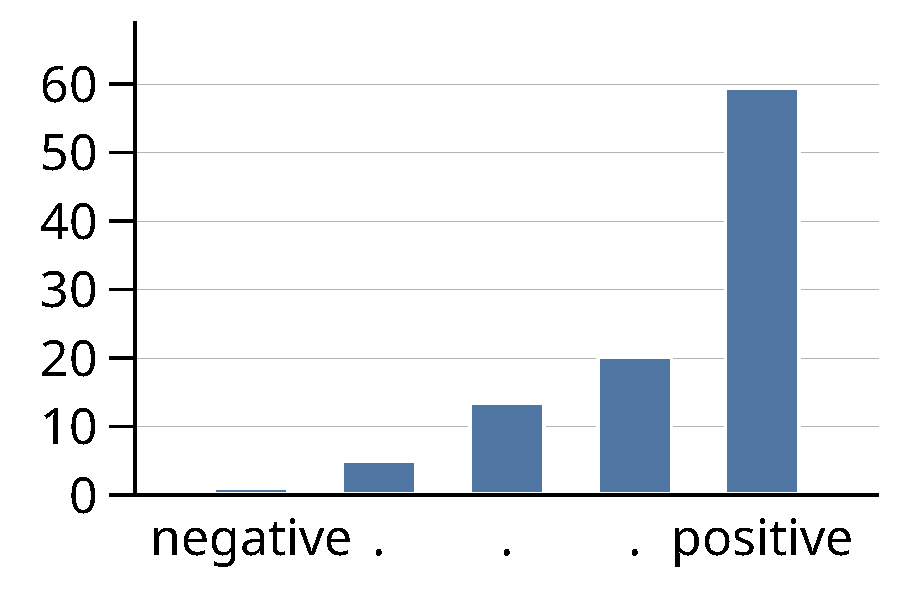
\includegraphics[width=1\linewidth]{descriptives/fig_ment_sf.pdf}
    \caption{\code{sf}: Limited socially due to health \phantom{text}}
    \label{fig:sf}
\end{subfigure}\hfill%
    \caption[Histogram of health variables used in the factor model]
    {Histogram of physical and mental health variables used in the factor model} \par \footnotesize
    \vspace{5pt} 
    Notes: Graphs depict proportion of categories so that they sum up to 100. 
    Labels recoded to order from `negative' to `positive' in terms of health outcome, independently of specific wording.
    For a detailed description on question wording, framing and recoding, see Table~\ref{tab:health_fact_varname_and_questions}.
    \label{fig:main_multifig_phys}
\end{figure}














\begingroup
% The \begingroup ... \endgroup pair ensures values of spacing 
% parameters only affect this particular table, and not any
% subsequent ones in the document.
\renewcommand{\arraystretch}{1.2} % Default value: 1
\renewcommand{\thefootnote}{\alph{footnote}}
\newcommand{\inlinecode}{\texttt}

\newcommand{\rowgroupemph}[1]{\hspace{-1em}\textbf{#1}}
%\newcommand{\rowgroupemph}[1]{\hspace{0em}\underline{#1}}
\begin{table}[tb]
    \centering
    \begin{adjustbox}{max width=.9\textwidth}
        \begin{threeparttable}
            \caption{Overview of module health module from individual questionnaire}
            \label{tab:health_fact_varname_and_questions}
            %\begin{tabularx}{\textwidth}{lX X}
            \begin{tabularx}{\textwidth}{>{\hspace{+1em}}l l >{\raggedright\arraybackslash}X}
                \toprule
                Category            & Variable               & Question \\
                \midrule
                \rowgroupemph{Physical Health Domain} \\ 
                Physical Function 1  & \code{pf1~(ple0004)} & $^{(b)}$When you have to climb several flights of stairs on foot, does your health limit you greatly, somewhat, or not at all?                                                                                      \\
                Physical Function 2  & \code{pf2~(ple0005)} & $^{(b)}$And what about other demanding everyday activities, such as when you have to lift something heavy or do something requiring physical mobility: Does your health limit you greatly, somewhat, or not at all? \\
                General Health       & \code{gh~~(ple0008)} & $^{(c,rev)}$How would you describe your current health?                                                                                                                                                                 \\
                Bodily Pain          & \code{bp~~(ple0030)} & $^{(a)}$have severe physical pain?                                                                                                                                                                                  \\
                Role Physical 1      & \code{rp1~(ple0031)} & $^{(a)}$feel that due to physical health problems you achieved less than you wanted to at work or in everyday activities?                                                                                           \\
                Role Physical 2      & \code{rp2~(ple0032)} & $^{(a)}$feel that due to physical health problems you were limited in some way at work or in everyday activities?                                                                                                   \\[3ex]
                \midrule
                \rowgroupemph{Mental Health Domain} \\
                Stress               & \code{st~~(ple0026)} & $^{(a,e)}$feel rushed or pressed for time?                                                                                                                                                                            \\
                Mental Health 1      & \code{mh1~(ple0027)} & $^{(a)}$feel down and gloomy?                                                                                                                                                                                       \\
                Mental Health 2      & \code{mh2~(ple0028)} & $^{(a,rev)}$feel calm and relaxed?                                                                                                                                                                                      \\
                Vitality             & \code{vt~~(ple0029)} & $^{(a,rev)}$feel energetic?                                                                                                                                                                                             \\
                Role Emotional 1     & \code{re1~(ple0033)} & $^{(a)}$feel that due to mental health or emotional problems you achieved less than you wanted to at work or in everyday activities?                                                                                \\
                Role Emotional 2     & \code{re2~(ple0034)} & $^{(a)}$feel that due to mental health or emotional problems you carried out your work or everyday tasks less thoroughly than usual?                                                                                \\
                Social Function      & \code{sf~~(ple0035)} & $^{(a)}$feel that due to physical or mental health problems you were limited socially, that is, in contact with friends, acquaintances, or relatives?                                                               \\
                \bottomrule
            \end{tabularx}
            %        \begin{tablenotes}[para,flushleft]
                \begin{tablenotes}[para,flushleft]   
                    \footnotesize
                    \item Notes: This table shows an overview of the questions used in the factor models to construct the physical 
                    and mental health scores. Names of input variables from \code{pl} dataset in parenthesis.\\
                    \item a: Categorical variable with 5 levels (1: \textit{Always} to 5: \textit{Never}) and time framed as \textit{previous four weeks}.\\
                    \item b: Categorical variable with 3 levels (1: \textit{Greatly} to 3: \textit{Not at all}) and no explicit time frame.\\
                    \item c: Categorical variable with 5 levels (1: \textit{Very good} to 5: \textit{Bad}) and time framed as \textit{currently}.\\
                    \item rev: Categories order reversed so lower values are `negative' and higher values are `positive' health outcomes.\\
                    \item e: \code{st} is not included SF-12 methodology and, for better comparability, also not in the alternative factor model, but 
                    displayed here for completeness.
                \end{tablenotes}
            \end{threeparttable}
        \end{adjustbox}
    \end{table}
    
    \endgroup













% -------------------------------------------------------------------------------------------------
% Robustness Checks ----
% -------------------------------------------------------------------------------------------------
\chapter{Robustness Checks}

\section{Model specification variation}
\label{modelspecificationvariation}
% -------------------------------------------------------------------------------------------------
% input figures with histograms of mental and physical health questions ----
% -------------------------------------------------------------------------------------------------




\newcommand{\vlgwnlog}{Gross Wealth (log)}                   % gw_nlog
\newcommand{\vlnwnlog}{Net Wealth (neglog)}                  % nw_nlog
\newcommand{\vlgw}{Gross Wealth (k€, winsored)}              % gw
\newcommand{\vlnw}{Net Wealth (k€, winsored)}                % nw
\newcommand{\vlexpue}{Unemployment exp. (months)}            % expue
\newcommand{\vlexpft}{Full-Time exp. (months)}               % expft
\newcommand{\vlemplstatus}{Employment Status of Individual}  % empl_status
\newcommand{\vllaborearns}{Individual Labor Earnings}        % labor_earns
\newcommand{\vlcardioev}{Cardiopathy}                        % cardio_ev
\newcommand{\vldepresev}{Depression}                         % depres_ev


% -------------------------------------------------------------------------------------------------
%  {\vlgwnlog}{Gross Wealth (log)}                   % gw_nlog
% -------------------------------------------------------------------------------------------------
% -------------------------------------------------------------------------------------------------
\begin{figure}[htb!]
    \centering
    \begin{subfigure}{0.45\textwidth}
        \caption{Gross Wealth (log)\qquad Models: P1\tsub{a} / M1\tsub{a}}
        \includegraphics[width=.95\linewidth]{../../output/figures/csdid2/f_robust/ep1_gw_nlog.pdf}
        \label{sfig:ep1_gw_nlog}
    \end{subfigure}
    \begin{subfigure}{0.45\textwidth}
        \caption{Gross Wealth (log)\qquad Models: P1\tsub{b} / M1\tsub{b}}
        \includegraphics[width=.95\linewidth]{../../output/figures/csdid2/f_robust/ep2_gw_nlog.pdf}
        \label{sfig:ep2_gw_nlog}
    \end{subfigure}
    \begin{subfigure}{0.45\textwidth}
        \caption{Gross Wealth (log)\qquad Models: P1\tsub{c} / M1\tsub{c}}
        \includegraphics[width=.95\linewidth]{../../output/figures/csdid2/f_robust/ep3_gw_nlog.pdf}
        \label{sfig:ep3_gw_nlog}
    \end{subfigure}
    \begin{subfigure}{0.45\textwidth}
        \caption{Gross Wealth (log)\qquad Models: P1\tsub{d} / M1\tsub{d}}
        \includegraphics[width=.95\linewidth]{../../output/figures/csdid2/f_robust/ep4_gw_nlog.pdf}
        \label{sfig:ep4_gw_nlog}
    \end{subfigure}
    \caption{Varying model specification}
    \label{fig:ep_gw_nlog}
    \fnote{Notes: Replications with $\log(Gross~Wealth)$ as response variable with  different specifications to check for model dependence.\\
        Models P1\tsub{a} and M1\tsub{a} include not-yet-treated (as well as never-treated) as comparison units. \\ 
        Models P1\tsub{b} and M1\tsub{b} do not include any covariates. \\
        Models P1\tsub{c} and M1\tsub{c} include covariates and are weighted by the inverse probability of remaining in the SOEP, to account for sample attrition might have differential impact over the wealth
        distribution. \\
        Models P1\tsub{d} and M1\tsub{d} are balanced, estimated with people present from 2002 to 2020.
        %                todo: this part to main text body 
        The coefficients are stable across models and similar to those obtained from the 
        main specifications P1 and M1. The estimated coefficients of the mental
        health domain are consistently higher than those of the physical domain. 
        Coefficients (and standard errors) already transformed to represent the effect in percentage terms. 
        The same results are also presented in \cref{tab:t_cmp_gw_nlog}.}
\end{figure}

%S[table-format=1.3, table-space-text-post ={***}]
% -------------------------------------------------------------------------------------------------
%\newcolumntype{p}{>{\columncolor{cp}}S}
%\newcolumntype{P}{>{}S[table-number-alignment = left]}
%\newcolumntype{P}{>{\columncolor{cp}}S[table-number-alignment = left]}
%\newcolumntype{M}{>{\columncolor{cm}}S[table-number-alignment = left]}
\begin{table}[htb!]
    \begin{adjustbox}{max width=\textwidth}
        \begin{threeparttable}
            \scriptsize
            \caption{Varying model specification}
            \label{tab:t_cmp_gw_nlog}
            %            \setlength{\tabcolsep}{12pt}
            \begin{tabular}{l*{4}{P}*{4}{M}}
                \toprule
                & \multicolumn{4}{l}{Physical Health} & \multicolumn{4}{l}{Mental Health}                             \\ %\cmidrule(lr){2-5} \cmidrule(lr){6-9} 
                & \multicolumn{4}{l}{Gross Wealth (log)} & \multicolumn{4}{l}{Gross Wealth (log)}                             \\ \cmidrule(lr){2-5} \cmidrule(lr){6-9} 
                & {(P1\tsub{a})}       & {(P1\tsub{b})}       & {(P1\tsub{c})}        & {(P1\tsub{d})}        & {(M1\tsub{a})}       & {(M1\tsub{b})}       & {(M1\tsub{c})}        & {(M1\tsub{d})}       \\
                & (\%)       & (\%)               & (\%)                & (\%)                & (\%)       & (\%)               & (\%)                &  (\%)              \\
                \midrule%
                
SimpleATT           &      -0.079\sym{**} &      -0.073\sym{**} &      -0.081\sym{***}&      -0.106\sym{*}  &      -0.085\sym{***}&      -0.081\sym{***}&      -0.095\sym{***}&      -0.111\sym{**} \\
                    &      (0.02)         &      (0.02)         &      (0.02)         &      (0.04)         &      (0.02)         &      (0.02)         &      (0.02)         &      (0.04)         \\
Pre\_avg             &       0.026         &       0.031         &       0.009         &       0.048         &       0.020         &       0.005         &      -0.010         &       0.007         \\
                    &      (0.04)         &      (0.04)         &      (0.04)         &      (0.05)         &      (0.03)         &      (0.03)         &      (0.04)         &      (0.05)         \\
Post\_avg            &      -0.090\sym{**} &      -0.089\sym{**} &      -0.099\sym{**} &      -0.111\sym{**} &      -0.107\sym{***}&      -0.101\sym{***}&      -0.116\sym{***}&      -0.113\sym{**} \\
                    &      (0.03)         &      (0.03)         &      (0.03)         &      (0.04)         &      (0.03)         &      (0.03)         &      (0.03)         &      (0.04)         \\
tm10                &      -0.012         &       0.013         &      -0.014         &       0.040         &       0.034         &       0.020         &      -0.038         &       0.111         \\
                    &      (0.09)         &      (0.09)         &      (0.09)         &      (0.10)         &      (0.07)         &      (0.07)         &      (0.08)         &      (0.09)         \\
tm8                 &       0.068         &       0.073         &       0.033         &       0.074         &       0.004         &      -0.025         &      -0.030         &      -0.048         \\
                    &      (0.05)         &      (0.05)         &      (0.06)         &      (0.07)         &      (0.05)         &      (0.05)         &      (0.05)         &      (0.07)         \\
tm6                 &       0.013         &       0.007         &      -0.016         &       0.032         &       0.010         &      -0.002         &       0.004         &      -0.036         \\
                    &      (0.04)         &      (0.04)         &      (0.04)         &      (0.05)         &      (0.03)         &      (0.03)         &      (0.04)         &      (0.05)         \\
tm4                 &       0.034\sym{*}  &       0.031\sym{*}  &       0.032\sym{*}  &       0.044         &       0.031\sym{*}  &       0.028         &       0.025         &       0.000         \\
                    &      (0.02)         &      (0.02)         &      (0.02)         &      (0.02)         &      (0.02)         &      (0.01)         &      (0.02)         &      (0.03)         \\
tp0                 &      -0.022         &      -0.014         &      -0.021         &      -0.033         &      -0.011         &      -0.010         &      -0.022         &      -0.028         \\
                    &      (0.01)         &      (0.01)         &      (0.01)         &      (0.02)         &      (0.01)         &      (0.01)         &      (0.01)         &      (0.02)         \\
tp2                 &      -0.038\sym{*}  &      -0.026         &      -0.036         &      -0.073\sym{*}  &      -0.032         &      -0.031         &      -0.046\sym{*}  &      -0.049         \\
                    &      (0.02)         &      (0.02)         &      (0.02)         &      (0.03)         &      (0.02)         &      (0.02)         &      (0.02)         &      (0.03)         \\
tp4                 &      -0.099\sym{***}&      -0.095\sym{***}&      -0.099\sym{***}&      -0.099\sym{*}  &      -0.102\sym{***}&      -0.103\sym{***}&      -0.118\sym{***}&      -0.090\sym{*}  \\
                    &      (0.03)         &      (0.03)         &      (0.03)         &      (0.04)         &      (0.03)         &      (0.02)         &      (0.03)         &      (0.04)         \\
tp6                 &      -0.133\sym{***}&      -0.118\sym{***}&      -0.126\sym{***}&      -0.133\sym{**} &      -0.122\sym{***}&      -0.114\sym{***}&      -0.130\sym{***}&      -0.120\sym{**} \\
                    &      (0.04)         &      (0.03)         &      (0.04)         &      (0.05)         &      (0.03)         &      (0.03)         &      (0.03)         &      (0.05)         \\
tp8                 &      -0.148\sym{***}&      -0.136\sym{**} &      -0.147\sym{**} &      -0.136\sym{*}  &      -0.169\sym{***}&      -0.150\sym{***}&      -0.167\sym{***}&      -0.166\sym{**} \\
                    &      (0.04)         &      (0.04)         &      (0.05)         &      (0.06)         &      (0.04)         &      (0.04)         &      (0.04)         &      (0.05)         \\
tp10                &      -0.111\sym{*}  &      -0.131\sym{**} &      -0.148\sym{**} &      -0.177\sym{**} &      -0.125\sym{**} &      -0.122\sym{**} &      -0.139\sym{**} &      -0.161\sym{**} \\
                    &      (0.05)         &      (0.05)         &      (0.05)         &      (0.06)         &      (0.05)         &      (0.04)         &      (0.05)         &      (0.06)         \\
tp12                &      -0.081         &      -0.103         &      -0.114         &      -0.127         &      -0.187\sym{**} &      -0.176\sym{***}&      -0.188\sym{***}&      -0.178\sym{**} \\
                    &      (0.07)         &      (0.06)         &      (0.07)         &      (0.07)         &      (0.06)         &      (0.05)         &      (0.06)         &      (0.06)         \\
\midrule
Pretrend $\chi^2$ (df)&       26.71         &       28.00         &       22.61         &       36.19         &       16.45         &       19.18         &       20.14         &       65.88         \\
Pretrend p-value    &  22 (0.222)         &  22 (0.176)         &  22 (0.424)         &  28 (0.138)         &  22 (0.793)         &  22 (0.634)         &  22 (0.574)         &  28 (0.000)         \\
Covariates          &                     &$\checkmark$         &$\checkmark$         &$\checkmark$         &                     &$\checkmark$         &$\checkmark$         &$\checkmark$         \\
Inv.Pr(stay)        &                     &                     &$\checkmark$         &                     &                     &                     &$\checkmark$         &                     \\
Balanced            &                     &                     &                     &$\checkmark$         &                     &                     &                     &$\checkmark$         \\
\bottomrule

            \end{tabular}
            \begin{tablenotes}[para,flushleft]
                \vspace*{-\baselineskip} {\raggedleft*~$p<0.05$,~**~$p<0.01$,~***~$p<0.001$\\}
                Notes: Replications with $\log(Gross~Wealth)$ as response variable with different specifications to check for model dependence.  
                Wild Bootstrap standard error in parenthesis. 
                \item Models P1\tsub{a} and M1\tsub{a} include not-yet-treated (as well as never-treated) as comparison units. \\ 
                \item Models P1\tsub{b} and M1\tsub{b} do not include any covariates. \\
                \item Models P1\tsub{c} and M1\tsub{c} include covariates and are weighted by the inverse probability of remaining in the SOEP, to account for sample attrition might have differential impact over the wealth
                distribution. \\
                \item Models P1\tsub{d} and M1\tsub{d} are balanced, estimated with people present from 2002 to 2020.
                %                todo: this part to main text body 
                The coefficients are stable across models and similar to those obtained from the 
                main specifications P1 and M1. 
                The covariates included are gender, age spline, federal state residence, legal disability, marital status, and years of education.
                Coefficients (and standard errors) already transformed to represent the effect in percentage terms. 
                For a visual representation of the same results see \cref{fig:ep_gw_nlog}.
            \end{tablenotes}
        \end{threeparttable}
    \end{adjustbox}
\end{table} % todo: include number in balanced model
% -------------------------------------------------------------------------------------------------
% -------------------------------------------------------------------------------------------------



% -------------------------------------------------------------------------------------------------
% tab:diff_treat_rule ----
% -------------------------------------------------------------------------------------------------
\begin{table}[htbp!]
    \centering \
    \begin{adjustbox}{max width=1\textwidth}
        \begin{threeparttable}
            \scriptsize
            \caption{Table of results with different treatment rule}
            \label{tab:diff_treat_rule}
            \setlength{\tabcolsep}{6pt}
            \begin{tabular}{l PPPP MMMM}
                \toprule
                & \multicolumn{4}{l}{Physical Health} & \multicolumn{4}{l}{Mental Health}                             \\ \cmidrule(lr){2-5} \cmidrule(lr){6-9} 
                & \multicolumn{2}{l}{(neg)log} & \multicolumn{2}{l}{level} & \multicolumn{2}{l}{(neg)log} & \multicolumn{2}{l}{level} \\ \cmidrule(lr){2-3} \cmidrule(lr){4-5} \cmidrule(lr){6-7} \cmidrule(lr){8-9} 
                & {gross (\%)} & {net (\%)$^1$} & {gross} & {net} & {gross (\%)} & {net (\%)$^1$} & {gross} & {net}           \\ 
                & {(P1\tsub{r})}       & {(P2\tsub{r})}       & {(P3\tsub{r})}        & {(P4\tsub{r})}        & {(M1\tsub{r})}       & {(M2\tsub{r})}       & {(M3\tsub{r})}        & {(M4\tsub{r})}       \\
                \midrule%
                
SimpleATT           &       -3.44\sym{*}  &       -2.77         &       -4.07\sym{*}  &       -4.47\sym{**} &       -7.36\sym{***}&       -8.40\sym{***}&       -4.52\sym{*}  &       -3.97\sym{*}  \\
                    &      (1.70)         &      (2.39)         &      (1.75)         &      (1.56)         &      (1.62)         &      (2.13)         &      (1.80)         &      (1.62)         \\
Pre average             &        1.60         &        4.74         &        3.47         &        2.86         &        3.00         &        4.75         &        1.53         &        2.16         \\
                    &      (2.24)         &      (3.41)         &      (2.12)         &      (1.92)         &      (2.42)         &      (3.12)         &      (2.73)         &      (2.26)         \\
Post average            &       -4.80         &       -3.25         &       -6.47\sym{*}  &       -6.75\sym{**} &       -9.66\sym{***}&      -10.74\sym{***}&       -6.37\sym{*}  &       -5.39\sym{*}  \\
                    &      (2.49)         &      (3.63)         &      (2.70)         &      (2.44)         &      (2.17)         &      (2.91)         &      (2.83)         &      (2.31)         \\
$\hat{\theta}_{es}(-10)$                &        6.04         &        9.38         &        5.62         &        5.11         &        3.22         &        5.53         &        1.15         &        3.89         \\
                    &      (4.67)         &      (7.28)         &      (4.00)         &      (3.72)         &      (5.05)         &      (6.71)         &      (5.40)         &      (4.76)         \\
$\hat{\theta}_{es}(-8)$                 &       -1.76         &        1.73         &        2.80         &        1.86         &        4.50         &        7.53         &        1.98         &        3.48         \\
                    &      (3.27)         &      (4.85)         &      (3.20)         &      (2.86)         &      (3.47)         &      (4.81)         &      (3.54)         &      (3.12)         \\
$\hat{\theta}_{es}(-6)$                 &        1.22         &        4.12         &        4.64\sym{*}  &        3.57\sym{*}  &        2.41         &        1.66         &        1.46         &        0.19         \\
                    &      (2.09)         &      (3.04)         &      (1.97)         &      (1.71)         &      (2.10)         &      (2.89)         &      (2.22)         &      (2.03)         \\
$\hat{\theta}_{es}(-4)$                 &        1.03         &        3.86\sym{*}  &        0.81         &        0.88         &        1.90         &        4.37\sym{**} &        1.54         &        1.09         \\
                    &      (1.12)         &      (1.63)         &      (0.95)         &      (0.86)         &      (1.13)         &      (1.50)         &      (0.97)         &      (0.86)         \\
$\hat{\theta}_{es}(0)$                 &       -0.69         &       -2.45         &       -0.77         &       -1.19         &       -2.41\sym{**} &       -2.76\sym{*}  &       -1.79\sym{*}  &       -1.36\sym{*}  \\
                    &      (0.77)         &      (1.34)         &      (0.74)         &      (0.73)         &      (0.80)         &      (1.16)         &      (0.71)         &      (0.69)         \\
$\hat{\theta}_{es}(2)$                 &       -2.56         &       -3.19         &       -3.42\sym{*}  &       -3.46\sym{*}  &       -4.14\sym{**} &       -5.10\sym{*}  &       -2.53         &       -2.49         \\
                    &      (1.58)         &      (2.50)         &      (1.51)         &      (1.39)         &      (1.53)         &      (2.28)         &      (1.51)         &      (1.42)         \\
$\hat{\theta}_{es}(4)$                 &       -3.94         &       -1.41         &       -4.77\sym{*}  &       -6.06\sym{**} &      -10.91\sym{***}&      -12.36\sym{***}&       -5.25\sym{*}  &       -5.30\sym{**} \\
                    &      (2.26)         &      (3.73)         &      (2.35)         &      (2.17)         &      (2.07)         &      (2.96)         &      (2.37)         &      (2.02)         \\
$\hat{\theta}_{es}(6)$                 &       -6.21\sym{*}  &       -3.57         &       -4.72         &       -5.79\sym{*}  &      -11.42\sym{***}&      -14.55\sym{***}&       -7.17\sym{*}  &       -6.24\sym{*}  \\
                    &      (2.79)         &      (4.39)         &      (2.93)         &      (2.51)         &      (2.46)         &      (3.35)         &      (3.01)         &      (2.78)         \\
$\hat{\theta}_{es}(8)$                 &       -7.76\sym{*}  &       -2.10         &       -6.49         &       -5.63         &      -13.42\sym{***}&      -14.26\sym{**} &       -7.64\sym{*}  &       -6.91\sym{*}  \\
                    &      (3.55)         &      (5.35)         &      (3.87)         &      (3.50)         &      (3.08)         &      (4.23)         &      (3.89)         &      (3.39)         \\
$\hat{\theta}_{es}(10)$                &       -5.71         &       -3.02         &      -10.44\sym{*}  &      -10.35\sym{*}  &      -12.58\sym{**} &      -11.91\sym{*}  &       -7.71         &       -6.59         \\
                    &      (4.18)         &      (6.35)         &      (5.29)         &      (4.45)         &      (3.95)         &      (4.91)         &      (5.20)         &      (4.63)         \\
$\hat{\theta}_{es}(12)$                &       -6.51         &       -6.88         &      -14.66\sym{*}  &      -14.77\sym{*}  &      -12.13\sym{*}  &      -13.50\sym{*}  &      -12.48         &       -8.83         \\
                    &      (6.02)         &      (7.54)         &      (6.82)         &      (5.94)         &      (4.74)         &      (6.13)         &      (6.52)         &      (5.44)         \\
\midrule
Obs                 &       {90,207}         &       {90,207}         &       {90,207}         &       {90,207}         &       {84,925}         &       {84,925}         &       {84,925}         &       {84,925}         \\
Pretrend $\chi^2$ (df)&  {24.8 (26)}         &  {18.1 (26)}         &  {36.2 (26)}         &  {38.9 (26)}         &  {23.4 (26)}         &  {29.9 (26)}         &  {36.6 (26)}         &  {31.6 (26)}         \\
Pretrend p-value    &       {0.529}         &       {0.872}         &       {0.088}         &       {0.050}         &       {0.608}         &       {0.272}         &       {0.081}         &       {0.205}         \\
\bottomrule
            \end{tabular}
            \begin{tablenotes}[para,flushleft]
                \vspace*{-\baselineskip} 
                {\raggedleft*~$p<0.05$,~**~$p<0.01$,~***~$p<0.001$ \\}
                Notes: Results of replicating the primary model with a different assignment rule. 
                Instead of having to experience a negative health outcome at least twice, people experiencing it 
                only once is already assigned to treatment. Further, the threshold is 1~Std.~Dev. instead of $1/2$ used in the main analysis. 
                In general, the results are similar, but consistently smaller than in the main analysis. The difference is
                around half to two thirds of estimations in the main results. The only model which is not strongly affected
                by these parameter changes is the one with gross wealth in logarithms as the response variable, M1\tsub{r} in the
                robustness checks and M1 in the main analysis. 
                The covariates included are gender, age spline, federal state residence, legal disability, marital status, and years of education.
                $^1$Coefficients (and standard errors) of log specifications are transformed to represent the effect in percentage terms, but
                such interpretation of the neglog transformation might be biased (see \cref{sec:transformcoefs})
                Wild Bootstrap standard error in parenthesis. 
                The main results are presented in \cref{tab:main_res_event} and the corresponding notes 
                on the procedure apply to this table equally. 
            \end{tablenotes}
        \end{threeparttable}
    \end{adjustbox}
\end{table}
% -------------------------------------------------------------------------------------------------
% -------------------------------------------------------------------------------------------------





% -------------------------------------------------------------------------------------------------
% figure: robustness checks (diff treat rule) ----
% -------------------------------------------------------------------------------------------------
\begin{figure}[ht!]
    \centering
    \begin{subfigure}{0.45\textwidth}
        \caption{Gross Wealth (log)\\(P1\tsub{r} / M1\tsub{r})}
        \includegraphics[width=.95\linewidth]{../../output/figures/csdid2/b_mcspcs/f_11_gw_nlog_1_ct1.pdf}
        \label{sfig:did_gw_nlog1ct1}
    \end{subfigure}
    \begin{subfigure}{0.45\textwidth}
        \caption{Net Wealth (neglog)\\(P2\tsub{r} / M2\tsub{r})}
        \includegraphics[width=.95\linewidth]{../../output/figures/csdid2/b_mcspcs/f_21_nw_nlog_1_ct1.pdf}
        \label{sfig:did_nw_nlog1ct1}
    \end{subfigure}
    \begin{subfigure}{0.45\textwidth}
        \caption{Gross Wealth (k€, winsored)\\(P3\tsub{r} / M3\tsub{r})}
        \includegraphics[width=.95\linewidth]{../../output/figures/csdid2/b_mcspcs/f_31_gw_1_ct1.pdf}
        \label{sfig:did_gw1ct1}
    \end{subfigure}
    \begin{subfigure}{0.45\textwidth}
        \caption{Net Wealth (k€, winsored)\\(P4\tsub{r} / M4\tsub{r})}
        \includegraphics[width=.95\linewidth]{../../output/figures/csdid2/b_mcspcs/f_41_nw_1_ct1.pdf}
        \label{sfig:did_nw1ct1}
    \end{subfigure}
    \caption{Event-study results with different treatment assignment rule}
    \label{fig:diff_treat_rule}
    \fnote{Notes: The results corresponding to this panel is presented in \cref{tab:diff_treat_rule}.
        The same notes apply to this figure. }
\end{figure}



% pcs_main        // Physical Health (oblique)
% gw_nlog         // Gross Wealth (log)
% gw              // Gross Wealth (k€, winsored)
% pcs_main        // Physical Health (oblique)
% empl_status     // Employment Status of Individual
% sats_health     // Satisfaction With Health
% mcs_main        // Mental Health (oblique)
% gw_nlog         // Gross Wealth (log)
% gw              // Gross Wealth (k€, winsored)
% mcs_main        // Mental Health (oblique)
% expue           // Unemployment exp. (months)
% sats_health     // Satisfaction With Health




\begin{figure}[htb!]
    % -------------------------------------------------------------------------------------------------
    % var: pcs_main         % Physical Health Domain
    % -------------------------------------------------------------------------------------------------
    % -------------------------------------------------------------------------------------------------
    \centering \setcounter{subfigure}{0}% Reset subfigure counter
    %%A: Physical Health Domain
    %\\ %%%%%%%%%%%%%%%%%%%%%%%%%%%%%%%%%%%%%%%%%%%%%%%%%%%%%%%%%%%%%%%%%%%%%%%%%%%%%%%%%%%%%%%%%%%
    \begin{subfigure}{0.32\textwidth}
        \caption{Physical Health (oblique)}
        \includegraphics[width=.95\linewidth]{../../output/figures/csdid2/h_descr/f_pcs_main_pcs_main_n1_win1.pdf}
        \label{sfig:fpcsmainpcsmain}
    \end{subfigure}
    \begin{subfigure}{0.32\textwidth}
        \caption{Gross Wealth (log)}
        \includegraphics[width=.95\linewidth]{../../output/figures/csdid2/h_descr/f_gw_nlog_pcs_main_n1_win1.pdf}
        \label{sfig:fgwnlogpcsmain}
    \end{subfigure}
    \begin{subfigure}{0.32\textwidth}
        \caption{Gross Wealth (k€, winsored)}
        \includegraphics[width=.95\linewidth]{../../output/figures/csdid2/h_descr/f_gw_pcs_main_n1_win1.pdf}
        \label{sfig:fgwpcsmain}
    \end{subfigure}
    \begin{subfigure}{0.32\textwidth}
        \caption{Mental Health (oblique)}
        \includegraphics[width=.95\linewidth]{../../output/figures/csdid2/h_descr/f_pcs_main_mcs_main_n1_win1.pdf}
        \label{sfig:fpcsmainmcsmain}
    \end{subfigure}
    \begin{subfigure}{0.32\textwidth}
        \caption{Unemployment exp. (months)}
        \includegraphics[width=.95\linewidth]{../../output/figures/csdid2/h_descr/f_expue_pcs_main_n1_win1.pdf}
        \label{sfig:fexpuepcsmain}
    \end{subfigure}
    \begin{subfigure}{0.32\textwidth}
        \caption{Satisfaction With Health}
        \includegraphics[width=.95\linewidth]{../../output/figures/csdid2/h_descr/f_sats_health_pcs_main_n1_win1.pdf}
        \label{sfig:fsatshealthpcsmain}
    \end{subfigure}
    % start main caption
    \caption{Development of selected variables from event study (Physical Health Domain)}
    \label{fig:inlevelspcsmain}
    \fnote{Panels depict the evolution of selected variables for the
        treated group (in red) and the untreated (in blue). In panel (a), one can see that, on average, the untreated do experience a strong direct impact at $e=0$
        but it recovers to the previous values in the next period ($e=2$), while the treated recovers only
        slightly and carry on on a downward trend. In panel (d), one can see the cross effect on the other health domain. That is,
        how does the shock in the one health dimension affect the other health dimension. Whiskers depict the 99\% confidence interval. \\
        Notes:\\
        - a: The untreated group, by definition, are not
        assigned a ``event year'', so their event is set as the year when they experience their worst
        health outcome, albeit still below the threshold. The actual DiD procedure do not impute any treatment
        year for the untreated, but for this visualization, one has to set a date or assign randomly and any
        choice would have some drawbacks. This choice is able depicting the evolution of people on limit of treatment assignment.\\
        - b: The vertical line depict the last period before (imputed) treatment taking place.\\
        - c: To avoid sample composition affecting the interpretation of these figures, the sample is restricted to a balanced panel.}
\end{figure}

\begin{figure}[htb!]
    % -------------------------------------------------------------------------------------------------
    % var: mcs_main         % Mental Health Domain
    % -------------------------------------------------------------------------------------------------
    % -------------------------------------------------------------------------------------------------
    \centering \setcounter{subfigure}{0}% Reset subfigure counter
    %%A: Mental Health Domain
    %\\ %%%%%%%%%%%%%%%%%%%%%%%%%%%%%%%%%%%%%%%%%%%%%%%%%%%%%%%%%%%%%%%%%%%%%%%%%%%%%%%%%%%%%%%%%%%
    \begin{subfigure}{0.32\textwidth}
        \caption{Mental Health (oblique)}
        \includegraphics[width=.95\linewidth]{../../output/figures/csdid2/h_descr/f_mcs_main_mcs_main_n1_win1.pdf}
        \label{sfig:fmcsmainmcsmain}
    \end{subfigure}
    \begin{subfigure}{0.32\textwidth}
        \caption{Gross Wealth (log)}
        \includegraphics[width=.95\linewidth]{../../output/figures/csdid2/h_descr/f_gw_nlog_mcs_main_n1_win1.pdf}
        \label{sfig:fgwnlogmcsmain}
    \end{subfigure}
    \begin{subfigure}{0.32\textwidth}
        \caption{Gross Wealth (k€, winsored)}
        \includegraphics[width=.95\linewidth]{../../output/figures/csdid2/h_descr/f_gw_mcs_main_n1_win1.pdf}
        \label{sfig:fgwmcsmain}
    \end{subfigure}
    \begin{subfigure}{0.32\textwidth}
        \caption{Physical Health (oblique)}
        \includegraphics[width=.95\linewidth]{../../output/figures/csdid2/h_descr/f_mcs_main_pcs_main_n1_win1.pdf}
        \label{sfig:fmcsmainpcsmain}
    \end{subfigure}
    \begin{subfigure}{0.32\textwidth}
        \caption{Unemployment exp. (months)}
        \includegraphics[width=.95\linewidth]{../../output/figures/csdid2/h_descr/f_expue_mcs_main_n1_win1.pdf}
        \label{sfig:fexpuemcsmain}
    \end{subfigure}
    \begin{subfigure}{0.32\textwidth}
        \caption{Satisfaction With Health}
        \includegraphics[width=.95\linewidth]{../../output/figures/csdid2/h_descr/f_sats_health_mcs_main_n1_win1.pdf}
        \label{sfig:fsatshealthmcsmain}
    \end{subfigure}
    % start main caption
    \caption{Development of selected variables from event study (Mental Health Domain)}
    \label{fig:inlevelsmcsmain}
    \fnote{Notes: points a: b: and c: of \cref{fig:inlevelspcsmain} also apply, as well as similar interpretation of each panels.
        Emphasis here to panel (e), showing a nice example of the effect taking place after not only parallel but equal pre-trend.}
\end{figure}



\begin{figure}
    \centering
    {Kaplan--Meier survival estimates}\par
    \includegraphics[width=0.7\linewidth]{../../output/figures/attrition/kpme_surv_nw_qile_age}
    \caption{Survival analysis of SOEP participants by wealth quintiles}
    \label{fig:kpmesurvnwqileage}
    \fnote{
        Notes: This graph evidentiates the gradient in panel attrition by wealth levels.
        It depicts an unadjusted survival estimate of participation length for each quintile of 
        age-adjusted gross wealth.  While the four upper quintile groups show a similar survival rate, 
        those in the bottom quintile are less likely to remain as long in the SOEP.
        The graph suggests that the differential attrition 
        rate is stronger in the first 5 years. From then on, the curves evolve parallel to one another. 
        For this analysis, SOEP's entering yeard is used, including if it happened before 2002. Those that dropped out
        before 2002 (from when on wealth data are available) are not considered for this examination. 
        Data source: SOEPv37.
        }
\end{figure}






% -------------------------------------------------------------------------------------------------
% -------------------------------------------------------------------------------------------------
% -------------------------------------------------------------------------------------------------
% -------------------------------------------------------------------------------------------------
% PCS_DEF ----
\chapter{Replications based on the SF-12 method}%
%
% -------------------------------------------------------------------------------------------------
% -------------------------------------------------------------------------------------------------
% -------------------------------------------------------------------------------------------------
\begin{figure}
    % -------------------------------------------------------------------------------------------------
    % var: pcs_def         % Physical Health Domain
    % -------------------------------------------------------------------------------------------------
    % -------------------------------------------------------------------------------------------------
    \centering \setcounter{subfigure}{0}% Reset subfigure counter
    \renewcommand{\thesubfigure}{P\alph{subfigure}}
    Physical Health Domain
    \\ %%%%%%%%%%%%%%%%%%%%%%%%%%%%%%%%%%%%%%%%%%%%%%%%%%%%%%%%%%%%%%%%%%%%%%%%%%%%%%%%%%%%%%%%%%%
    \begin{subfigure}{0.32\textwidth}
        \caption{Physical Health (oblique)}
        \includegraphics[width=.95\linewidth]{../../output/figures/csdid2/h_descr/f_pcs_def_pcs_def_n1_win1.pdf}
        \label{sfig:fpcsdefpcsdef}
    \end{subfigure}
    \begin{subfigure}{0.32\textwidth}
        \caption{Gross Wealth (log)}
        \includegraphics[width=.95\linewidth]{../../output/figures/csdid2/h_descr/f_gw_nlog_pcs_def_n1_win1.pdf}
        \label{sfig:fgwnlogpcsdef}
    \end{subfigure}
    \begin{subfigure}{0.32\textwidth}
        \caption{Gross Wealth (k€, winsored)}
        \includegraphics[width=.95\linewidth]{../../output/figures/csdid2/h_descr/f_gw_pcs_def_n1_win1.pdf}
        \label{sfig:fgwpcsdef}
    \end{subfigure}
    \begin{subfigure}{0.32\textwidth}
        \caption{Mental Health (oblique)}
        \includegraphics[width=.95\linewidth]{../../output/figures/csdid2/h_descr/f_pcs_def_mcs_def_n1_win1.pdf}
        \label{sfig:fpcsdefmcsdef}
    \end{subfigure}
    \begin{subfigure}{0.32\textwidth}
        \caption{Unemployment exp. (months)}
        \includegraphics[width=.95\linewidth]{../../output/figures/csdid2/h_descr/f_expue_pcs_def_n1_win1.pdf}
        \label{sfig:fexpuepcsdef}
    \end{subfigure}
    \begin{subfigure}{0.32\textwidth}
        \caption{Satisfaction With Health}
        \includegraphics[width=.95\linewidth]{../../output/figures/csdid2/h_descr/f_sats_health_pcs_def_n1_win1.pdf}
        \label{sfig:fsatshealthpcsdef}
    \end{subfigure}
%    % start def caption
%    \caption{Development of selected variables from event study (Physical Health Domain)}
%    \label{fig:inlevelspcsdef}
%    \fnote{}
%\end{figure}
%\begin{figure}[htb!]
%    % -------------------------------------------------------------------------------------------------
%    % var: mcs_def         % Mental Health Domain
%    % -------------------------------------------------------------------------------------------------
%    % -------------------------------------------------------------------------------------------------
    \centering \setcounter{subfigure}{0}% Reset subfigure counter
    \renewcommand{\thesubfigure}{M\alph{subfigure}}
    Mental Health Domain
    \\ %%%%%%%%%%%%%%%%%%%%%%%%%%%%%%%%%%%%%%%%%%%%%%%%%%%%%%%%%%%%%%%%%%%%%%%%%%%%%%%%%%%%%%%%%%%
    \begin{subfigure}{0.32\textwidth}
        \caption{Mental Health (oblique)}
        \includegraphics[width=.95\linewidth]{../../output/figures/csdid2/h_descr/f_mcs_def_mcs_def_n1_win1.pdf}
        \label{sfig:fmcsdefmcsdef}
    \end{subfigure}
    \begin{subfigure}{0.32\textwidth}
        \caption{Gross Wealth (log)}
        \includegraphics[width=.95\linewidth]{../../output/figures/csdid2/h_descr/f_gw_nlog_mcs_def_n1_win1.pdf}
        \label{sfig:fgwnlogmcsdef}
    \end{subfigure}
    \begin{subfigure}{0.32\textwidth}
        \caption{Gross Wealth (k€, winsored)}
        \includegraphics[width=.95\linewidth]{../../output/figures/csdid2/h_descr/f_gw_mcs_def_n1_win1.pdf}
        \label{sfig:fgwmcsdef}
    \end{subfigure}
    \begin{subfigure}{0.32\textwidth}
        \caption{Physical Health (oblique)}
        \includegraphics[width=.95\linewidth]{../../output/figures/csdid2/h_descr/f_mcs_def_pcs_def_n1_win1.pdf}
        \label{sfig:fmcsdefpcsdef}
    \end{subfigure}
    \begin{subfigure}{0.32\textwidth}
        \caption{Unemployment exp. (months)}
        \includegraphics[width=.95\linewidth]{../../output/figures/csdid2/h_descr/f_expue_mcs_def_n1_win1.pdf}
        \label{sfig:fexpuemcsdef}
    \end{subfigure}
    \begin{subfigure}{0.32\textwidth}
        \caption{Satisfaction With Health}
        \includegraphics[width=.95\linewidth]{../../output/figures/csdid2/h_descr/f_sats_health_mcs_def_n1_win1.pdf}
        \label{sfig:fsatshealthmcsdef}
    \end{subfigure}
    % start main caption
    \caption{Development of selected variables based on SF-12 method}
    \label{fig:inlevelsmcsdef}
    \fnote{Notes: Replication of \cref{fig:inlevelspcsmain,fig:inlevelsmcsmain} using PCS and MCS following the SF-12 method.
    Here one can observe the negative cross-effect in \subref{sfig:fpcsdefmcsdef} and \subref{sfig:fmcsdefpcsdef} where the adverse outcome 
    in one dimension impacts the other dimension in the opposite direction. The pre-treatment trend, specially in \subref{sfig:fexpuepcsdef} 
    and \subref{sfig:fexpuemcsdef}, are less supportive of the parallel trends assumption than in the alternative method.
    Same considerations regarding the ``treatment date'' of the untreated stated in the notes of  \cref{fig:inlevelspcsmain} apply here as well.}
\end{figure}





% ---------------------------------------------------------------------------------------------------------------------
% Validation with objective health diagnoses
% ---------------------------------------------------------------------------------------------------------------------
\begin{figure}[tb!]
    \centering
    \begin{subfigure}{0.45\textwidth}
        \caption{Depression}
        \includegraphics[width=.95\linewidth]{../../output/figures/csdid2/c_othervars/f_2_depres_ev_1o2_def.pdf}
    \end{subfigure}
    \begin{subfigure}{0.45\textwidth}
        \caption{Sleep Disorder}
        \includegraphics[width=.95\linewidth]{../../output/figures/csdid2/c_othervars/f_2_sleep_ev_1o2_def.pdf}
    \end{subfigure}
    \caption{Replication of validation of mental health diagnoses with orthogonal health scores} 
    \label{fig:csdid_hltdiag_rep}
    \fnote{Notes: This replication aims to show that also using orthogonal health scores, the effect follows 
        a similar in both domains, similar to using oblique scores. 
        Response variables are binary indicators of being ever diagnosed with the respective condition.
        Panels have different scale on the y-axis. Whiskers depict the 95\% confidence interval}
\end{figure}








































% -------------------------------------------------------------------------------------------------
% figure: SF-12 default pcs mcs
% -------------------------------------------------------------------------------------------------
\begin{figure}[ht!]
    \centering
    \begin{subfigure}{0.45\textwidth}
        \caption{Gross Wealth (log)\\(M1\tsub{sf12} / P1\tsub{sf12})}
        \includegraphics[width=.95\linewidth]{../../output/figures/csdid2/b_mcspcs/f_12_gw_nlog_1o2_ct2.pdf}
        \label{sfig:did_sf12_a}
    \end{subfigure}
    \begin{subfigure}{0.45\textwidth}
        \caption{Net Wealth (neglog)\\(M2\tsub{sf12} / P2\tsub{sf12})}
        \includegraphics[width=.95\linewidth]{../../output/figures/csdid2/b_mcspcs/f_22_nw_nlog_1o2_ct2.pdf}
        \label{sfig:did_sf12_b}
    \end{subfigure}
    \begin{subfigure}{0.45\textwidth}
        \caption{Gross Wealth (k€, winsored)\\(M3\tsub{sf12} / P3\tsub{sf12})}
        \includegraphics[width=.95\linewidth]{../../output/figures/csdid2/b_mcspcs/f_32_gw_1o2_ct2.pdf}
        \label{sfig:did_sf12_c}
    \end{subfigure}
    \begin{subfigure}{0.45\textwidth}
        \caption{Net Wealth (k€, winsored)\\(M4\tsub{sf12} / P4\tsub{sf12})}
        \includegraphics[width=.95\linewidth]{../../output/figures/csdid2/b_mcspcs/f_42_nw_1o2_ct2.pdf}
        \label{sfig:did_sf12_d}
    \end{subfigure}
    \caption{Replication of main analysis with SF-12 scores}
    \label{fig:did_sf12}
    \fnote{Notes: These panels are a visual representation of the table of coefficients presented in \cref{tab:coefs_sf12}. 
        Post-treatment, the effects are in line with those obtained in the main analysis. Pre-treatment, in contrast, seems 
        to be less supportive of the parallel trends assumptions, including in the primary specifications with log-transformed 
        gross wealth (P1\tsub{sf12} and M1\tsub{sf12}). To what extend this is driven by the particular treatment rule or
        whether an artifact from the sf12 or from the alternative scores computes could be a matter of further inquiry.
        To what extend should be, a priori, expected that the trends remain parallel 8 or 10 years prior to treatment 
        is also worth considering. 
    Whiskers depict the 95\% confidence interval.}
\end{figure}



\begin{table}[htbp!]
    \centering
    \begin{adjustbox}{max width=\textwidth}
        \begin{threeparttable}       
            \caption{Table of coefficients of models based on the SF-12 methodology}
            \label{tab:coefs_sf12} % \setlength{\tabcolsep}{4pt}
            \begin{tabular}{l*4{P}*4{M}}
                \toprule
                & \multicolumn{4}{l}{Physical Health}   & \multicolumn{4}{l}{Mental Health}     \\ \cmidrule(lr{1em}){2-5} \cmidrule(lr{1em}){6-9}
                & \multicolumn{2}{l}{(neg)log}               & \multicolumn{2}{l}{level} & \multicolumn{2}{l}{(neg)log} & \multicolumn{2}{l}{level} \\ \cmidrule(lr{1em}){2-3} \cmidrule(lr{1em}){4-5} \cmidrule(lr{1em}){6-7} \cmidrule(lr{1em}){8-9} 
                & {gross (\%)} & {net (\%)$^1$} & {gross} & {net} & {gross (\%)} & {net (\%)$^1$} & {gross} & {net}               \\
                & {(P1\tsub{sf12})}  & {(P2\tsub{sf12})}            & {(P3\tsub{sf12})}  & {(P4\tsub{sf12})}              & {(M1\tsub{sf12})}  & {(M2\tsub{sf12})}            & {(M3\tsub{sf12})}  & {(M4\tsub{sf12})}              \\  
                \midrule
                
SimpleATT           &       -6.12\sym{**} &       -5.78         &       -8.39\sym{***}&       -7.47\sym{***}&      -10.94\sym{***}&      -14.56\sym{***}&       -5.85\sym{*}  &       -5.50\sym{**} \\
                    &      (2.10)         &      (2.88)         &      (2.27)         &      (2.03)         &      (1.93)         &      (2.45)         &      (2.29)         &      (2.06)         \\
Pre average             &        3.81         &        4.61         &        4.65         &        4.34         &        9.25\sym{*}  &       11.62\sym{*}  &        6.61         &        5.30         \\
                    &      (3.55)         &      (4.88)         &      (3.61)         &      (3.10)         &      (4.11)         &      (5.34)         &      (4.40)         &      (3.53)         \\
Post average            &       -8.55\sym{**} &       -7.75\sym{*}  &      -10.77\sym{***}&       -9.69\sym{***}&      -12.58\sym{***}&      -17.18\sym{***}&       -7.29\sym{*}  &       -6.72\sym{*}  \\
                    &      (2.69)         &      (3.43)         &      (2.93)         &      (2.59)         &      (2.40)         &      (2.99)         &      (3.10)         &      (2.66)         \\
$\hat{\theta}_{es}(-10)$                &        1.63         &        3.27         &        7.50         &        6.36         &       24.71\sym{*}  &       19.85         &       15.82         &       15.35\sym{*}  \\
                    &      (8.42)         &     (10.85)         &      (8.31)         &      (6.69)         &     (10.76)         &     (13.79)         &      (9.54)         &      (7.41)         \\
$\hat{\theta}_{es}(-8)$                 &        9.54         &       10.56         &        5.30         &        5.86         &        8.29         &       15.61         &        7.26         &        4.74         \\
                    &      (6.03)         &      (7.97)         &      (5.40)         &      (4.52)         &      (5.83)         &      (8.57)         &      (6.80)         &      (5.98)         \\
$\hat{\theta}_{es}(-6)$                 &        2.53         &        2.56         &        3.09         &        2.99         &        2.36         &        6.34         &        0.59         &       -1.09         \\
                    &      (3.35)         &      (4.61)         &      (3.28)         &      (2.80)         &      (3.39)         &      (4.48)         &      (3.85)         &      (3.21)         \\
$\hat{\theta}_{es}(-4)$                 &        1.74         &        2.28         &        2.70\sym{*}  &        2.15         &        3.04         &        5.35\sym{**} &        2.74         &        2.20         \\
                    &      (1.57)         &      (2.28)         &      (1.22)         &      (1.18)         &      (1.63)         &      (2.06)         &      (1.46)         &      (1.30)         \\
$\hat{\theta}_{es}(0)$                 &       -0.76         &       -1.21         &       -2.53\sym{**} &       -2.48\sym{**} &       -3.31\sym{**} &       -5.12\sym{***}&       -1.90         &       -1.64         \\
                    &      (1.16)         &      (1.72)         &      (0.87)         &      (0.79)         &      (1.05)         &      (1.48)         &      (1.00)         &      (0.93)         \\
$\hat{\theta}_{es}(2)$                 &       -1.04         &       -1.60         &       -5.01\sym{**} &       -4.57\sym{**} &       -6.07\sym{***}&       -7.59\sym{***}&       -3.44         &       -2.96         \\
                    &      (1.86)         &      (2.64)         &      (1.68)         &      (1.60)         &      (1.62)         &      (2.21)         &      (1.92)         &      (1.75)         \\
$\hat{\theta}_{es}(4)$                 &       -5.91\sym{*}  &       -6.89         &       -8.65\sym{***}&       -7.47\sym{***}&      -12.91\sym{***}&      -15.48\sym{***}&       -6.84\sym{**} &       -7.12\sym{**} \\
                    &      (2.50)         &      (3.60)         &      (2.48)         &      (2.22)         &      (2.24)         &      (2.81)         &      (2.65)         &      (2.39)         \\
$\hat{\theta}_{es}(6)$                 &       -8.04\sym{*}  &       -7.62         &       -9.62\sym{**} &       -8.11\sym{**} &      -16.46\sym{***}&      -21.73\sym{***}&       -7.07\sym{*}  &       -7.56\sym{*}  \\
                    &      (3.04)         &      (4.09)         &      (3.27)         &      (2.91)         &      (2.55)         &      (3.38)         &      (3.39)         &      (3.09)         \\
$\hat{\theta}_{es}(8)$                 &      -10.67\sym{**} &       -7.57         &      -11.22\sym{**} &       -9.51\sym{**} &      -18.27\sym{***}&      -22.44\sym{***}&       -7.45         &       -6.66         \\
                    &      (3.88)         &      (4.98)         &      (3.76)         &      (3.51)         &      (3.24)         &      (4.06)         &      (4.29)         &      (3.95)         \\
$\hat{\theta}_{es}(10)$                &      -16.84\sym{***}&      -13.48\sym{*}  &      -18.96\sym{***}&      -16.75\sym{***}&      -15.39\sym{***}&      -22.25\sym{***}&       -9.75         &       -8.58         \\
                    &      (4.20)         &      (5.78)         &      (5.17)         &      (4.70)         &      (4.01)         &      (4.78)         &      (5.42)         &      (4.84)         \\
$\hat{\theta}_{es}(12)$                &      -15.30\sym{**} &      -14.97\sym{*}  &      -19.40\sym{**} &      -18.95\sym{**} &      -14.62\sym{**} &      -23.61\sym{***}&      -14.56\sym{*}  &      -12.53\sym{*}  \\
                    &      (4.99)         &      (6.79)         &      (6.71)         &      (5.88)         &      (5.06)         &      (5.89)         &      (6.77)         &      (5.98)         \\
\midrule
N                   &    {92,239}         &    {92,239}         &    {92,239}         &    {92,239}         &    {89,112}         &    {89,112}         &    {89,112}         &    {89,112}         \\
Unique N            &    {17,943}         &    {17,943}         &    {17,943}         &    {17,943}         &    {17,663}         &    {17,663}         &    {17,663}         &    {17,663}         \\
Pretrend $\chi^2$ (df)& {27.5 (22)}         & {24.5 (22)}         & {37.8 (22)}         & {37.8 (22)}         & {32.8 (22)}         & {27.1 (22)}         & {17.9 (22)}         & {17.6 (22)}         \\
Pretrend p-value    &     {0.193}         &     {0.322}         &     {0.019}         &     {0.019}         &     {0.065}         &     {0.208}         &     {0.709}         &     {0.732}         \\
\bottomrule
% &
            \end{tabular}%
            \begin{tablenotes}[para,flushleft]%
                \vspace*{-\baselineskip}
                {\raggedleft*~$p<0.05$,~**~$p<0.01$,~***~$p<0.001$\\}
                Notes: This results are a replication of \cref{tab:main_res_event} based on the SF-12 methodology for construction PCS and MCS. 
                Wild Bootstrap standard error in parenthesis. 
                A visual representation of this results are depicted in \cref{fig:did_sf12}
                $^1$Coefficients (and standard errors) of log specifications are transformed to represent the effect in percentage terms, but
                such interpretation of the neglog transformation might be biased (see \cref{sec:transformcoefs})
            \end{tablenotes}
        \end{threeparttable}
    \end{adjustbox}
\end{table}
% -------------------------------------------------------------------------------------------------
% end table 
% -------------------------------------------------------------------------------------------------





%

%
%\begin{figure}[htb!]
    \centering
    \begin{subfigure}{0.495\textwidth}
        \caption{Gross Wealth (log)}
        \includegraphics[width=.95\linewidth]{../../output/figures/csdid2/e_cs_twfe/c_gw_nlog_pcs_main_1o2_main_pb0.pdf}
        \label{sfig:olscsgwnlogpcsmain}
    \end{subfigure}
    \begin{subfigure}{0.495\textwidth}
        \caption{Net Wealth (neglog))}
        \includegraphics[width=.95\linewidth]{../../output/figures/csdid2/e_cs_twfe/c_nw_nlog_pcs_main_1o2_main_pb0.pdf}
        \label{sfig:olscsnwnlogpcsmain}
    \end{subfigure}
    \begin{subfigure}{0.495\textwidth}
        \caption{Gross Wealth (k€, winsored)}
        \includegraphics[width=.95\linewidth]{../../output/figures/csdid2/e_cs_twfe/c_gw_pcs_main_1o2_main_pb0.pdf}
        \label{sfig:olscsgwpcsmain}
    \end{subfigure}
    \begin{subfigure}{0.495\textwidth}
        \caption{Net Wealth (k€, winsored)}
        \includegraphics[width=.95\linewidth]{../../output/figures/csdid2/e_cs_twfe/c_nw_pcs_main_1o2_main_pb0.pdf}
        \label{sfig:olscsnwpcsmain}
    \end{subfigure}
    \caption{Comparison of $DiD_{DR}$ with TWFE specification (Physical Health Domain)} 
    \label{fig:twfe_cs_pcs_main}
    \fnote{%
    Notes: All models refer to the treatment analysis in the physical health domain.
    Whiskers depict the 95th confidence interval. 
    In the logarithm specifications, the models display similar results, although 
    with less precision in the CS specification. 
    In the specification in levels, the results differ considerably. The 
    TWFE would suggest a much stronger effect, but the nearly straight 
    line from pre-treatment to post-treatment ATT's, would indicate that 
    treated people were already in a different wealth accumulation path and 
    the differences post treatment would likely not be interpreted as an effect of health degradation. 
    This could suggest that the DiD\textsubscript{DR} does a good job at
    balancing the groups via the re-weighting step, as well as avoiding 
    the ``forbidden comparisons''. 
    }
\end{figure}




\begin{figure}[htb!]
    \centering
    \begin{subfigure}{0.495\textwidth}
        \caption{Gross Wealth (log)}
        \includegraphics[width=.95\linewidth]{../../output/figures/csdid2/e_cs_twfe/c_gw_nlog_mcs_main_1o2_main_pb0.pdf}
        \label{sfig:olscsgwnlogmcsmain}
    \end{subfigure}
    \begin{subfigure}{0.495\textwidth}
        \caption{Net Wealth (neglog))}
        \includegraphics[width=.95\linewidth]{../../output/figures/csdid2/e_cs_twfe/c_nw_nlog_mcs_main_1o2_main_pb0.pdf}
        \label{sfig:olscsnwnlogmcsmain}
    \end{subfigure}
    \begin{subfigure}{0.495\textwidth}
        \caption{Gross Wealth (k€, winsored)}
        \includegraphics[width=.95\linewidth]{../../output/figures/csdid2/e_cs_twfe/c_gw_mcs_main_1o2_main_pb0.pdf}
        \label{sfig:olscsgwmcsmain}
    \end{subfigure}
    \begin{subfigure}{0.495\textwidth}
        \caption{Net Wealth (k€, winsored)}
        \includegraphics[width=.95\linewidth]{../../output/figures/csdid2/e_cs_twfe/c_nw_mcs_main_1o2_main_pb0.pdf}
        \label{sfig:olscsnwmcsmain}
    \end{subfigure}
    \caption{Comparison of $DiD_{DR}$ with TWFE specification (Mental Health Domain)} 
    \par \footnotesize \raggedright
    \vspace{5pt} 
    Notes: All models refer to the treatment analysis in the mental health domain. 
    Whiskers depict the 95th confidence interval. 
    In the mental health domain, the two models are much more in line with one another than when comparing them in the
    physical domain (see \cref{fig:twfe_cs_pcs_main})
    \label{fig:twfe_cs_mcs_main}
\end{figure}
%
%


